\section{Introduction}
During the development of the visual system neurons must make precise synaptic connections with each other, producing neural circuits that are capable of generating visual guided behaviours. As these connections change, so too must the patterns of activity that are distributed across these populations of neurons.  A major goal of this thesis is to understand how the developmental trajectory of such population activity is influenced by changes in the visual environment because these changes are likely to underlie any changes in behaviour.  A prerequisite of this is that features of population activity can be quantified in order understand how the underlying neural circuitry maybe altered. Therefore the aim of this first results chapter is to introduce methods and metrics to quantify the structure and dynamics of population in the tectum. These methods will be used in subsequent chapters to understand how EE modifies the development of population activity in the tectum.

One approach to studying the circuit architecture of the visual system is to record activity when the organism is in total darkness. This is because high levels of activity persists and correlated activity is likely to be seen between neurons that share a high degree of connectivity with each other rather that being driven by a common source, such as a visual stimulus.  As a result, previous studies have shown that spontaneous activity takes the form of discrete local populations of neurons known as neural assemblies which show spatiotemporally orchestrated patterns of coactivity (\cite{Miller2014}; \cite{Carrillo-Reid2015}). Importantly these same assemblies that are spontaneously active have been shown to be active during natural vision and correlate with certain behaviours (\cite{Miller2014}; \cite{Carrillo-Reid2015};  \cite{Stringer2019SpontaneousActivity}; \cite{Luczak2007}; \cite{Romano2015}). These observation has led to the suggestion that neural assemblies may be acting as the functional units of the brain and that spontaneous activity, due to network constraints, revisits preferred network states through "attractor-like" dynamics (\cite{Hebb1949}; \cite{Romano2015}; \cite{Yuste2015}, \cite{Marachlian2018PrinciplesTectum}). Therefore the structure of spontaneous activity can give insight into the underlying patterns of functional connectivity within the visual system allowing for the developmental trajectory of circuits in the visual system to be mapped (\cite{Avitan2017}; \cite{Pietri2017}).

However, automatically identifying and quantifying features of assemblies from population recordings can be challenging for a number of reasons. Firstly, the number of assemblies is not known \textit{a priori}. Secondly, an assembly's constituent neurons are noisy with not all neurons being recruited at every assembly activation and some neurons may fire independently from their assembly. Assemblies also show temporal overlap in their firing, making them difficult to distinguish from each other. Finally, some neurons may not be tightly coupled to an assembly at all and therefore their activity generates noise when clustering (\cite{Molter2018}; \cite{Diana2019BayesianAssemblies}).

Previous methods to identify assemblies have either relied upon dimensionality reduction techniques such as \gls{pca} followed by factor analysis, or spectral clustering methods to identify communities from graphical representations of the data (\cite{Lopes-dos-Santos2011}; \cite{Carrillo-Reid2015}; \cite{Romano2015}; \cite{Avitan2017}).  These methods can perform well in scenarios where there are clearly defined independent groups and that fire with low levels of noise (\cite{Molter2018}). However, as the complexity and noise within the data increases these techniques can lead to spurious conclusions as shown by ground truth validation tests (\cite{Diana2019BayesianAssemblies}). Furthermore, as these methods do not quantify the certainty over the assignment of a neuron to an assembly there is no way of knowing when neurons are likely to be miss-assigned.  To address these problems a member of our lab recently developed a new method which utilises a hierarchical model of assembly activity and Bayesian inference techniques. This method (\gls{bina}) has been shown to out perform previous methods in validation tests, even in scenarios where the level of noise is high (\cite{Diana2019BayesianAssemblies}). Unlike other existing methods it also uses a statistical framework that provides probabilistic estimates of assembly number, membership and activity. Therefore this method could be used to understand both the structure and dynamics of assemblies within the developing brain.

The aim of this chapter is to characterise the structure of population activity in the optic tectum at 7 \gls{dpf} when a fish is raised under normal laboratory conditions. At this age the optic tectum already possesses the neural circuitry required to engage in complex visually guided behaviour such as prey capture (\cite{Gahtan2005}; \cite{Bianco2015}). Consistent with previous studies I find that spontaneous activity is characterised by groups of synchronously firing neural assemblies (\cite{Romano2015}; \cite{Avitan2017}; \cite{Pietri2017}). Using the Bayesian inference method to quantify both the structure and dynamics of these assemblies reveals that the majority of assemblies are spatially compact and lateralised and that assembly structure and organisation correlates with assembly dynamics. This chapter therefore provides a description of population activity in the tectum that can be used to understand how this tectal circuitry develops and is shaped by the visual environment in subsequent chapters.

\section{Results}
\subsection{Calcium imaging of spontaneous activity in the optic tectum}
To study the how spontaneous population activity is organised within the optic tectum 7 \gls{dpf} larval zebrafish expressing \textit{nls-GCaMP6s} under a pan-neuronal promotor were imaged for ~1 hr in complete darkness. This imaging was performed using 2-photon microscope equipped with a resonant scanner and peizo lens holder enabled fast volumetric imaging of both tectal hemispheres at a rate of 4.8Hz per volume (\textbf{Figure \ref{fig:R1_F1}A-C}). Each volume consisted of 5 optical sections that were approximately 15$\mu$m apart giving a total imaging depth of 75 $\mu$m covering 75\% of the tectal volume.  Following image acquisition each slice was registered to itself, the cell bodies were were segmented from the registered mean images and the fluorescence signal for each cell was extracted with around 3000-4000 cells being segmented per fish, although not all of these were active (\textbf{Figure \ref{fig:R1_F1}D}). 

Whilst the on rate of GCaMP6s is relatively fast, the decay of the response is slow and is thought to be even slower when localized to the nucleus (\cite{Chen2013}; \cite{Vladimirov2014}). This is likely to cause artifactual correlations between neurons if the complete extent of the GCaMP6s signal is used for correlation analysis. For example, two neurons firing a few seconds apart would appear to be correlated due to the slow kinetics of the probe. To avoid such a scenario a \gls{hmm} was used to binarise the trace by identifying timepoints where there is maximum likelihood of the neuron being active (\cite{Diana2019BayesianAssemblies}). It is important to note that the inferred events do not correspond to individual action potentials but timepoints where there is maximum likelihood of the neuron being activate. This can be used to identify correlations between neurons. In addition, this model can also reconstruct the calcium signal (free from signal noise and drifting baseline) so that parameters such response amplitude and duration can still be estimated \textbf{(see Figure \ref{fig:R1_F1}E and \textbf{Materials and methods})}. Any traces that contained no calcium events throughout the duration of the recording were discarded.

\begin{figure}[!ht]
        \center{\includegraphics[width =  0.8\paperwidth]{Figures/R1_F1.pdf}}
        \caption[\label{fig:R1_F1} \textbf{Recording spontaneous activity from the optic tectum of the larval zebrafish.}]{\label{fig:R1_F1} \textbf{Recording spontaneous activity from the optic tectum of the larval zebrafish. (A)} 7\gls{dpf}	 zebrafish	 larvae	 expressing	 \emph{nls-GCaMP6s}	 were	 mounted	 in agarose	 and	 the spontaneous	neural	activity from	both	tectal	hemispheres	was imaged in a	single	plane using	a	 two	photon	microscope	in	 total	darkness	 for	one	hour. \textbf{(B)} A high resolution single slice through the center of the zebrafish brain with pan-neuronal expression of \emph{nls-GCaMP6s}. The optic tectum is a large bilateral structure sitting on the dorsal surface of the mindbrain (highlighted in blue).  \textbf{(C)} Imaging volumes consisted of 5 optical slices that were 15$\mu$m apart and were imaged at 4.8Hz per volume. \textbf{(D)} A mean image of tectal cells in a single optical slice with active cells segmented (highlighted in blue). \textbf{(E)}  The raw fluorescence signal for each cell (black) was binarised into time points where there was maximum likelihood of the neurons being active (red) using a hidden Markov model. This model also allowed for the calcium signal to be reconstructed (green). }
      \end{figure}
    
\subsection{Single neuron properties of neurons within the tectum}
Prior to understanding the interactions between neurons I wanted to determine how the firing properties of single neurons within the tectum because these may be affected by  both development and visual experience (\cite{Pietri2017}; \cite{Avitan2016}; \cite{Pratt2007HomeostaticCircuit}). Firstly, the number of active cells in each recording were estimated from the segmentation. Around 400-500 cells were found to be active in each optical slice meaning that the number of active cells in each volume was approximately 2257$\pm$188 (mean $\pm$ \gls{sd}) \textbf{(Figure \ref{fig:R1_F2}A}). The segmentation algorithm identifies neurons based on both morphology and correlated activity between pixels. This means that it mainly active cells are segmented, making it difficult to assess what proportion of cells in the tectum are active. However, manual counting of a couple of optical slices provided estimates that between 50-70\% of cells were spontaneously active within our recordings. 

\begin{figure}[!htb]
        \center{\includegraphics[width = 0.7\paperwidth]{Figures/R1_F2.pdf}}
        \caption[\label{fig:R1_F2}  \textbf{Response properties of spontaneously active neurons.}]{\label{fig:R1_F2}  \textbf{Properties of spontaneous active neurons in the optic tectum. (A)} The number of active cells in the optic tectum of all fish (n=8). Density plots for single neuron properties such as \textbf{(B)} Firing frequency (events/second), \textbf{(C)} response amplitude  ($\Delta$F/F) and \textbf{(D)} response duration (seconds). For all density plots the grey lines demonstrate the distribution for each fish and the the purple line represent the mean distribution across fish.}
      \end{figure}


In order to understand the distribution of firing properties of these active neurons a number of activity parameters were calculated. Firstly, the firing frequency was calculated from the binarised trace by counting the average number of active time-points per second for each neuron. It should be noted that this is only a rough estimate of firing frequency as there are likely to be far more spikes within a single time frame. Each fish was found to have a very similar sparse levels of activity where found across all fish with he majority of data centered around a mean across fish of 0.06 $\pm$ 10$^{-5}$ events/second and a tail that extended towards higher frequencies \textbf{(Figure \ref{fig:R1_F2}B}). Finally, by isolating each response from the inferred calcium signal the mean response amplitude and duration for each neuron could be calculated \textbf{(Figure \ref{fig:R1_F2}C-D}). Here response amplitude and duration are likely to reflect frequency and length of the underlying spike trains. Like firing frequency, all fish showed similar distributions for both response amplitude and duration with a mean of  0.75$\pm$ 0.018 $\Delta$F/F and 4.90$\pm$0.18 Seconds respectively. 


\subsection{Spontaneous activity is correlated in groups of spatially clustered neurons}

Having looked at the properties of single neurons I next  determined the spatiotemporal organisation of population activity. To do this, cell activity was plotted by time in a raster plot and the number of neurons at each time point were summed revealing that there were frames with a high degree of synchronous activity (\cite{Romano2015}). In order to understand if this structure could be explained by chance the time series for each neuron was circularly permuted. This has the effect of breaking the temporal structure between neurons yet preserving the firing statistics for each neuron.	By totalling up the activity at each frame there were a large number of frames where the coactivity in the data exceed	95\% of	the	distribution seen in the circularly permuted data (\textbf{Figure \ref{fig:R1_F3}A}). Thus the degree of pairwise correlated activity is more than would be expected by chance (\textbf{Figure \ref{fig:R1_F3}B}).

Synchronous events could be random, or they could represent the repeated spontaneous activation of the same groups of neuron in assemblies. To investigate this, a \gls{mi} between each frame was computed (\cite{Romano2015}):

\begin{equation}
    MI = 2\frac{\left | A \bigcap B \right |}{\left |  A + B\right |}
\end{equation}

where a and b are binary population vectors indicating the active and inactive neurons in a timeframe (1 = active, 0 = inactive). This gives a measure of similarity between the two frames where 1 indicates that two frames have all of the same neurons active and 0 indicates none (\textbf{Figure \ref{fig:R1_F3}C}). Pairwise MI values between frames were used to generate a similarity matrix for both significantly synchronous and non-synchronous events. For synchronous events the similarity matrix displayed an off diagonal block-like structure. Moving across a row of the matrix it was clear that similar frames occurred at multiple different points within the recording (\textbf{Figure \ref{fig:R1_F3}D}). These repeating frames did not always align vertically with those of other rows suggesting different populations of neuron were active at different times.  Importantly, this block-like structure was greatly reduced for non-synchronous events. This indicates that there are multiple different discrete populations of neurons that fire together synchronously and repeatedly throughout the recordings. 

\begin{figure}[!htb]
        \center{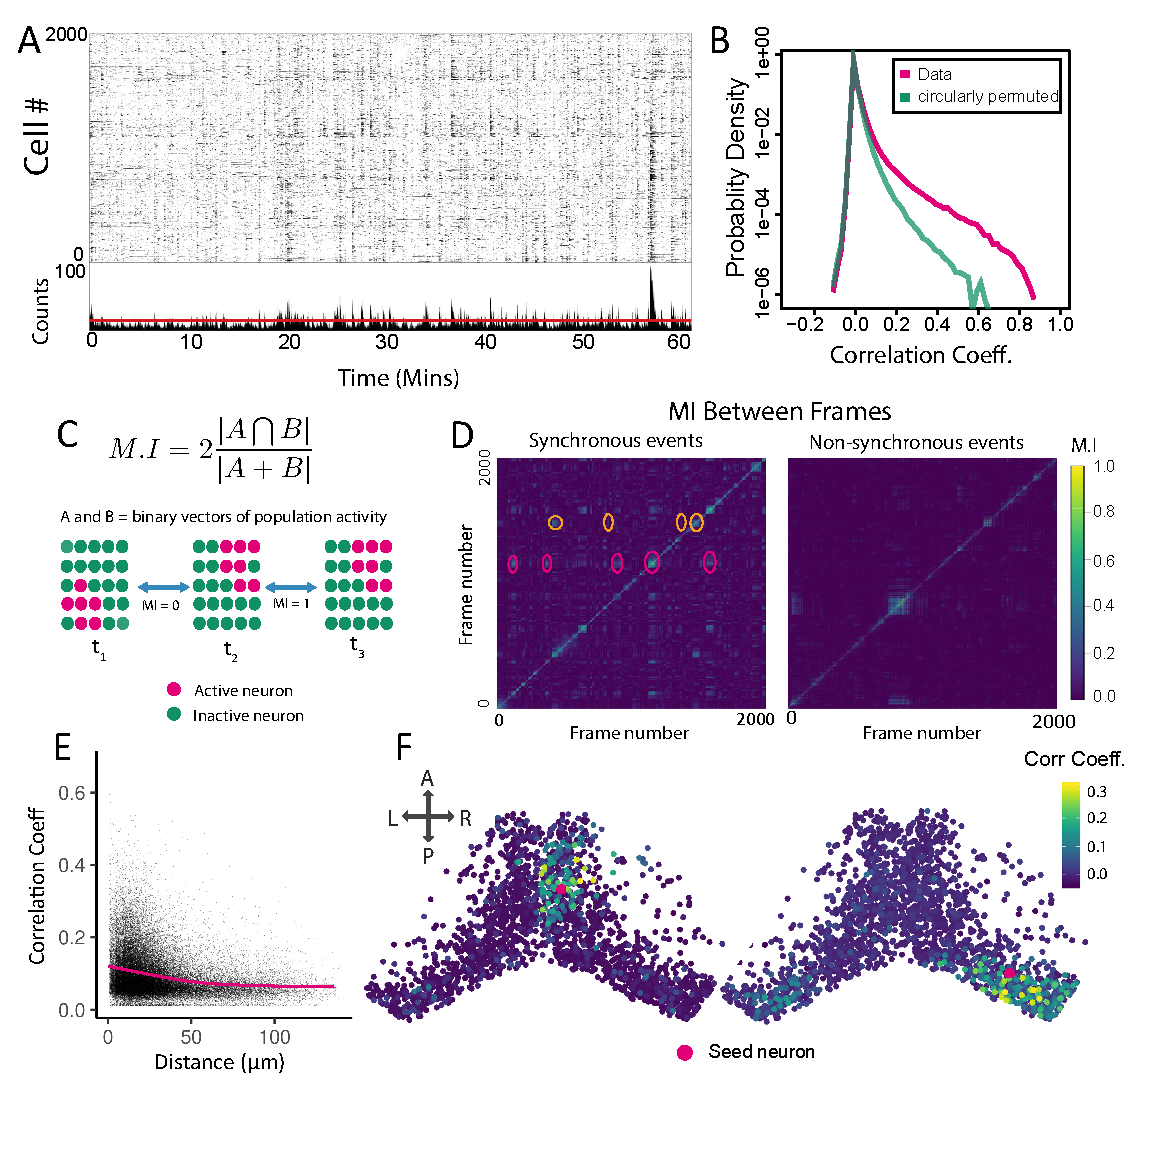
\includegraphics[width = 0.8\paperwidth]{Figures/R1_F3.pdf}}
        \caption[\label{fig:R1_F3} \textbf{Spatiotemporal organisation of spontaneous activity in the tectum.}]{\label{fig:R1_F3} \textbf{Spatiotemporal organisation of spontaneous activity in the tectum.  (A) Top:} Raster plot of population activity in the optic tectum. At certain time points the raster plot shows vertical banding, indicating that there is synchronous activity  across neurons. \textbf{Bottom:} The  number of cells that were active in each frame were counted. This shows frames where there are synchronous activation of cells which can not be explained by chance. The red line represents the 95\% of the distribution of coactive cells in a null model where the data was circularly permuted.  \textbf{(B)} The distribution of pairwise correlations in the tectum compared to the same null model as in A. \textbf{(C)} To understand if the same groups of neurons were repeatedly active throughout the recording, a \gls{mi} was calculated for all pairwise population vectors (ie. neurons active in each frame). This index ranged from 0 (no neurons in common - $t_{1} \ vs \ t_{2}$) to 1 (all neurons in common - $t_{2} \ vs \ t_{3}$). Where $t_{n}$ is a timeframe containing active and inactive neurons. \textbf{(D)} similarity matrices for synchronous and non-synchronous events indicating that synchronous events consist of groups of neurons that fire repeatedly throughout the recording. \textbf{(E)} A scatter plot of pairwise Pearsons correlation coefficient by euclidean distance between the neurons cell bodies. \textbf{(F)} Seed-based correlation maps with neurons colored by their correlation with the seed neuron (pink).}
      \end{figure}
      
To investigate the spatial organisation of this correlated activity within the tectum by calculating the correlation coefficents between each neuron and plotting these against the euclidean distance between their cell bodies.  This revealed that correlations decreased with increasing distance between neurons. (\textbf{Figure \ref{fig:R1_F3}E}). To visualise how these spatio-temporal correlations map onto the tectum the trace from single neuron was used as a "seed" for correlation with all other neurons. By colour-coding neurons according to correlation it can be seen that groups of correlated neurons are spatially clustered within the tectum \textbf{(Figure \ref{fig:R1_F3}F)}. Therefore, consistent with previous studies of the spontaneous population activity in the optic tectum these results suggest that spontaneous activity in the tectum is dominated by the synchronous activation of neural assemblies that are repeatedly active and spatially compact (\cite{Romano2015}; \cite{Avitan2017}; \cite{Pietri2017}).

\begin{figure}[!ht]
        \captionsetup{}
        \centering
        \center{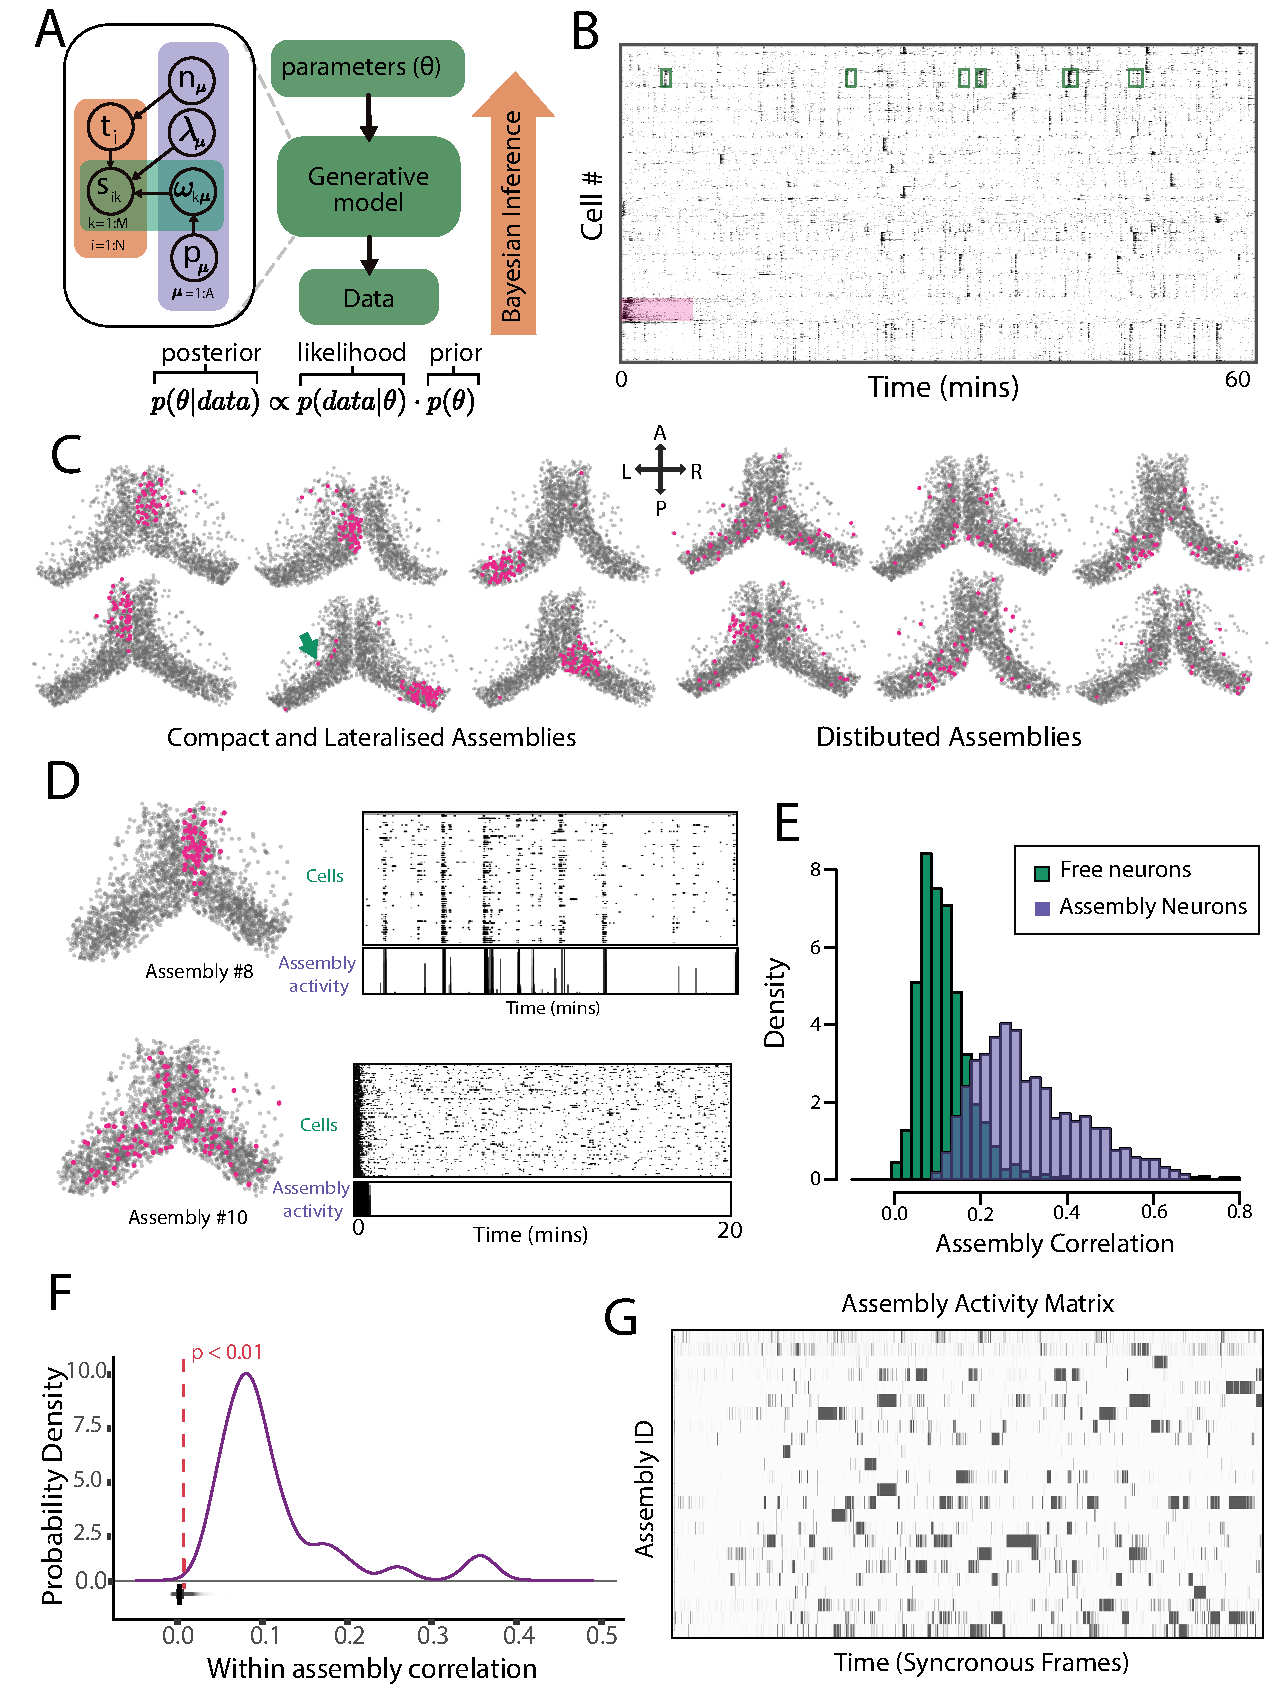
\includegraphics[width =  0.8\paperwidth]{Figures/R1_F4.jpg}}
            \caption[\label{fig:R1_F4} \textbf{Identifying neural assemblies using BINA.}] {\label{fig:R1_F4} \textbf{Identifying neural assemblies using BINA. (A)} A schematic explaining the components of the \gls{bina} method for identifying neural assemblies. The method contains a generative model which describes the assignment of neurons to assemblies and the firing properties of both those neurons and their assemblies. In this model neuronal activity of $N$ neurons is organised into $A$ assemblies over $M$ timeframes. Each neuron $i$ is given a single assembly assignment $t_{i}$ which is drawn from the categorical distribution. Here the probability of belonging to an assembly $\mu$ is given by $n_{\mu}$. \textit{(continued...)}}
            \end{figure}
            \clearpage
            \begin{figure}[!ht]
            \captionsetup{labelformat=adja-page}
            \ContinuedFloat
            \caption[]{Each assembly $\mu$ can occupy a ON/OFF state ($\omega_{k\mu} = \{0,1\}$) at each time $k$ which is drawn from a Bernoulli distribution with the assembly specific probability $P_{\mu}$. The parameters $\lambda\mu(1)$ and $\lambda\mu(0)$ represent the probabilities that neurons belonging an assembly μ fire when their assembly is active or inactive respectively. This generates the activity matrix $S_{ik}$ which represents the activity of each neuron $i$ and each timepoint $k$. To infer the values of these parameters, this matrix $S_{ik}$ is replaced by the actual spontaneous activity dataset (as shown in  \textbf{\ref{fig:R1_F3}A}).  Bayesian inference can then invert this generative process to give the posterior distribution of these parameter values given the spontaneous activity data. For clarity the priors have been excluded from this graphical representation of the generative model \textbf{(B)} A raster plot where neurons that has been sorted by assembly membership. This shows that assembly members fire together synchronously at multiple time points in the recording (an example is highlighted by the green boxes). Some assemblies where found to fire transiently at the beginning of the recording (highlighted in pink). Such assemblies are likely to be responding to the sound of the resonant scanner or the movement of the objective and were therefore excluded. \textbf{(C)} Assembly maps showing the spatial distribution of neural assemblies within the tectum. Some compact and lateralised assemblies had "satellite cells" in the contralateral hemisphere (green arrow). \textbf{(D) Top:} A compact assembly with its corresponding raster plot showing the timepoints that its cells are active. The plot of assembly activity shows time points that the assembly is active as inferred by BINA. \textbf{bottom:} An example of a distributed assembly that responding transiently at the beginning of the  recording. \textbf{(E)} Histograms showing the density of correlations (Pearsons) between either free neurons or assembly neurons with assembly activity. \textbf{F)} Within assembly correlation is significantly greater than randomly generated assemblies of the same size. \textbf{(G)} A raster plot showing the time points that each assembly was active, as inferred by the BINA \label{fig:R1_F4}}
    \end{figure}  
      
\clearpage
\subsection{Identifying neural assemblies in the tectum}
The findings above are consistent with previous findings showing that spontaneous activity in the tectum is organised into assemblies (\cite{Romano2015}; \cite{Avitan2017}; \cite{Pietri2017}). However, relatively little is known about the properties of these assemblies. For example, the number of neurons per assembly, the firing properties of the assemblies themselves, the behaviour of neurons within the assemblies and how assemblies interact with one another are not known. Because all of these features may be relevant for how the tectum encodes information and generates behaviour they are important metrics to quantify. For this purpose I used a Bayesian inference method (\gls{bina}) that has been previously shown to outperform other methods in validation tests. Furthermore, unlike other existing methods, \gls{bina} provides a statistical framework that quantifies the uncertainty of assembly parameters and can also infer the timepoints at which each assembly is active, allowing for the dynamics of the assembly to be quantified. 

Briefly \gls{bina} relies on a generative model to  describe the observed assembly activity through a set of unobserved (latent) features, $Z$, and model parameters, $\theta$. Contained within this model is the idea that there are neurons, these neurons are organised into assemblies and at each time point each assembly can occupy an activity state of ON or OFF. Neurons themselves can fire when their assembly in ON (synchronous firing) or when it is OFF (asynchronous firing) with certain probabilities. Therefore this model could generate data that resembles the population activity within the tectum given the correct model parameters (such as assembly membership, synchronous and asynchronous firing probabilities). The aim of Bayesian statistics is to invert this process and calculate the probability distribution of these parameters and latent variables conditional to the data using Bayes' theorem: 

\begin{align}
    \overset{\mathrm{Posterior}}{\overbrace{P(Z,\theta|\mathrm{data})}} \propto \overset{\mathrm{Data\;Likelihood}}{\overbrace{P(\mathrm{data},Z|\theta)}}\times \overset{\mathrm{Prior}}{\overbrace{P(\theta)}}
    \label{eq:bayes_theorem}
\end{align}

which expresses this probability in terms of the likelihood of observing the data (given the model parameters) and the prior distribution of the parameters which represents our a priori knowledge about the model. Calculating the full posterior distribution would require complete enumeration of all combinations of $\theta$ which is computationally unfeasible. Therefore \gls{bina} instead draws samples from this distribution using a Gibbs sampler allowing the posterior distribution to be approximated within a short period of time. This method therefore allows for the structure and dynamics of neural assemblies to be inferred from population data (for a graphical representation of the model see \textbf{Figure \ref{fig:R1_F4}A}).

 To apply this method to our data I first reduced the number of frames for each dataset by selecting only those frames where there were more than 15 neurons active. This is because it allowed for the sampler to reach convergence quicker whilst discarding frames where there is unlikely to be assembly activity. \gls{bina} initially assigns all neurons to an assigned to a potential cluster, including cells that may not actually belong to an assembly. As a result, there were a number of clusters which clearly were not assemblies. This is because they were not active at all within the duration of the recording, or contained very small numbers of neurons.  Such clusters do not fit the definition of an assembly ie. groups of neurons that fire together synchronously. Therefore only clusters which had an activity level > 0.5\% and a size larger than 5 neurons were used for subsequent analysis. In addition, only those cells that could be reliably assigned to an assembly in 99\% of the samples from the posterior were considered to belong to that assembly and any non-assigned cells were called "free neurons".

To demonstrate the validity of this method in identifying tectal assemblies in  a raster plot of neuronal activity was sorted by assembly membership. This revealed groups of neurons that were firing together at multiple different points within the recording (\textbf{Figure \ref{fig:R1_F4}B}). The spatial location of each assembly's constituent neurons were then superimposed back onto the tectum to show how they were spatially arranged (\textbf{Figure \ref{fig:R1_F4}C}). The majority of the assemblies were spatially compact, highly lateralised and found to tile the anterior posterior axis of the tectum.  Whilst most assemblies were compact there were a few assemblies that appeared to be more distributed, with constituent neurons spanning the complete extent of the tectum. However, many of these distributed assemblies were found only to be firing synchronously at the beginning of the recording suggesting that rather than being spontaneously active these assemblies were transiently responding to sensory input caused by the microscope starting to image. Therefore any assemblies showing these transient effects were excluded from further analysis because they are unlikely to reflect the preferred network states of the tectum (for examples \textbf{see Figure \ref{fig:R1_F4}B} and \textbf{Figure \ref{fig:R1_F4}D  assembly \# 10}).

Something that is inferred by the BINA method is the timepoints that each assembly is active (\textbf{Figure \ref{fig:R1_F4}D and G}). To ensure that assembly neurons were  correlated with their assembly and that the free neurons were not, the time correlation (Pearsons) between each assigned neuron and the activity of the assembly that it belongs to were calculated. Next the maximum correlation between each free neuron with each of the assemblies was taken. By plotting both these distributions together showed that assembly neurons are far more correlated with assembly activity than the free neurons. This suggests that BINA is able to identify only those neurons which are associated with assembly activity and that the free neurons are far less coupled to these populations.

To see if the retained assemblies could be explained by random groupings of cells within the tectum, null assemblies were generated by randomly picking the equivalent number of neurons to the assembly from all possible neurons in the tectum, this was repeated 2000 times. The mean within assembly correlation coefficent was then calculated for each assembly and its null assemblies by taking the average pairwise correlation between all of the assemblies constituent neurons. This showed that 100\% of assemblies exceed not just their own null distributions but also the null distributions for any assembly in the tectum with a p < 0.01 \textbf{(Figure \ref{fig:R1_F4}F)}. This demonstrates that the \gls{bina} clustering method is capable of isolating groups of neurons that fire together synchronously and reveals spatial structure that is not specified by parameters within the generative model. 
 
\subsection{Quantifying the structure and dynamics of tectal assemblies}
From using this Bayesian inference method it is possible to infer the identity of constituent neurons of an assembly and the timepoints where the assembly is active (\textbf{Figure \ref{fig:R1_F5}A-B}). This allows the structure and dynamics of the assemblies in the tectum to be obtained. To first understand how cells in the tectum were partitioned into these assemblies for all imaged fish. The average number of assemblies in each fish was 41$\pm$11 assemblies and ranged from 24 to 64 (\textbf{Figure \ref{fig:R1_F5}C}). Not all of the active neurons could be assigned reliably to an assembly; between 48\% - 70\% of active neurons were assigned with over 99\% probability to an assembly and the rest were considered to be "free neurons" (\textbf{Figure \ref{fig:R1_F5}D}).  For each fish the number of neurons that were recruited by each assembly showed similar broad distributions and had a mean across fish of 31$\pm$0.38 cells (\textbf{Figure \ref{fig:R1_F5}E}). 

By eye, assemblies in the tectum appeared to exhibit a high degree of spatial organisation by being both spatially compact and highly lateralised. To quantify these observations I generated metrics for both the spatial extent of the assembly and its lateralisation. Firstly, to measure the spatial extent of each assembly, an ellipse was fitted to the 2D distribution of its constituent neurons (visualised in \textbf{Figure \ref{fig:R1_F5}A}) This was achieved by calculating the two eigenvalues ($\xi_1$ and $\xi_2$) of the co-variance matrix of the XY neuronal coordinates within each assembly and then extension was quantified as:

\begin{align}
    E=\pi \sqrt{\xi_1\xi_2}
\end{align}

Lateralisation on the other hand was assessed using the following equation:

\begin{align}
    abs(LI) = abs\left(\frac{L - R}{L + R}\right)
\end{align}

where L is the number of cells within the left tectal hemisphere and R is the number of cells on the right. This gives a lateralisation index (LI) where the absolute value quantifies the degree of laterality which ranges from 0 (assembly is bilateral) to 1 (lateralised to a single hemisphere). To understand if assemblies were significantly compact and lateralised the same metrics were computed for 2000 topographic null models for each assembly. These null models were generated by randomly selecting the same number of neurons from all possible neuron locations in the tectum (spatial null models). This showed that for each fish 73\%$\pm$0.12  of assemblies were significantly compact (p<0.01) when compared to their own null model (\textbf{Figure \ref{fig:R1_F5}F}). Interestingly, each fish showed a slight bi-model distribution with a small number of assemblies occupying a larger spatial extent suggesting that there may be two separate types of assemblies within the tectum, those that are spatially compact and those that are more distributed. Likewise a large number of assemblies also showed high LI values with 78\%$\pm$0.01 being significantly lateralised (p<0.05) (\textbf{Figure \ref{fig:R1_F5}G}). Together these metrics demonstrate that these neural assemblies tend to exhibit a high degree of spatial organisation by being both compact and lateralised.

In addition to the structure of the assemblies I also wanted to understand their within-assembly dynamics. This is possible because within the \gls{bina} clustering method the assembly activity state is inferred as a latent variable within the model. This was used to estimate the frequency with which each assembly was active in events per minute (\textbf{Figure \ref{fig:R1_F5}H}) and most assemblies being active with a frequency of around 2.3$\pm$0.38 events/minute. One feature of assemblies is that their constituent cells can be noisy with not every cell firing when the assembly is active and cells also firing when their assembly is inactive (See \textbf{Figure \ref{fig:R1_F5}B}). This behaviour of neurons within each assembly can be quantified using two probability values: 1) synchrony, which is the probability that a neuron fires when its assembly is active and 2) asynchrony, which is the probability that a neuron fires when its assembly is inactive. All fish showed similar shaped distributions for synchrony with a mean value of 0.2$\pm$0.02, whereas asynchronous firing showed a tighter distribution with much smaller values than synchronous firing of 0.007$\pm$0.0008, indicating that assemblies neurons are far more likely to fire with their assembly rather than in isolation(\textbf{Figure \ref{fig:R1_F5}I-J}). Finally, assemblies in all fish showed significantly greater within assembly correlation when compared to assemblies containing random groupings of assembly neurons 99\%$\pm$0.09 (p < 0.01)(\textbf{Figure \ref{fig:R1_F5}K}). 



\begin{figure}[!ht]
        \center{\includegraphics[width =  0.77\paperwidth]{Figures/R1_F5.jpg}}
            \caption[\label{fig:R1_F5} \textbf{Characterising assembly structure and dynamics}]{\label{fig:R1_F5} \textbf{Characterising assembly structure and dynamics} \textbf{(A)} Parameters quantifying the structure of assemblies can be calculated from the spatial maps of assemblies such as spatial extent which is calculated by fitting an ellipse to its 2D distribution. \textbf{(B)} A plot showing the activity of the constituent neurons of the assembly relative to the the time points that the assembly is active (inferred from the model). This illustrates that not every neuron fires with the assembly every time and neurons can also be active when the assembly is inactive. \textbf{(C)} A bar plot showing the number of assemblies in each fish.  \textbf{(D)} A bar plot showing the percentage of neurons that can be assigned to an assembly with 99\% confidence, these assigned neurons were celled assembly neurons. Any neurons that did not meet this requirement, along with any neurons that belonged to excluded assemblies were called free neurons. \textbf{(E)} A density plot showing the distribution of assembly size in terms of the number of neurons. Grey lines represent single fish and purple thick line is the mean distribution across fish. \textbf{(F)} Density plots for the 2D spatial extent of all assemblies for each fish (orange) compared to their spatial null model (green). \textbf{(G)} Density plots of lateral index for all assemblies for each fish compered to their spatial null models. \textbf{(H)} Density plot of assembly firing frequency. \textbf{(I)} Density plot of synchrony, the probability that a neuron fires when its assembly is active. \textbf{(J)} Density plot of asynchrony which is the probability that a neuron fires when its assembly is in active. \textbf{(K)} Density plot of within assembly correlation for each fish compeared null models.}
      \end{figure}


\subsection{The relationship between assembly structure and dynamics}
Based on the observation that neural assemblies can occupy a range of firing properties I next asked whether these dynamic properties of an assembly could be related to its physical structure. For example, one possibility is that the firing rate of an assembly may be related to its size or compactness. To investigate this possibility correlation (Spearmans rank) was computed pairwise for all assembly parameters. This revealed a number of interesting correlations between structural parameters and  functional parameters. For example, negative correlation was seen between assembly size (number of neurons) and both synchrony and asynchrony parameters whereas a small positive correlation was seen between an assembly's lateral index and its firing frequency (\textbf{Figure \ref{fig:R1_F6}A-B}). Plotting these comparisons as scatter plots showed non-linear relationships between parameters of assembly structure and dynamics. Some of these relationships such as the one between assembly firing frequency and lateral index appeared to be very weakly related. Therefore to understand the relationship more fully a bootstrapping procedure was applied to each correlated pair by recomputing the correlation on subsampled data (20\% of the original dataset size) and was repeated for 20000 iterations. This produced empirical distributions for the correlation values. This showed that assembly size had a strong-moderate negative correlations with synchrony (rho = -0.63 $\pm$ 0.06) and asynchrony (rho = -0.47 $\pm$ 0.08) whereas lateral index and assembly firing frequency showed a weaker positive correlation of (rho =0.37 $\pm$ 0.06). This indicates that the physical structure of the assembly is correlated with its firing frequency and the coupling of neurons within the assembly. 


\begin{figure}[!ht]
        \center{\includegraphics[width =  0.8\paperwidth]{Figures/R1_F6.pdf}}
            \caption[\label{fig:R1_F6} \textbf{Correlation between assembly structure and assembly dynamics}]{\label{fig:R1_F6}\textbf{Correlation between assembly structure and assembly dynamics} \textbf{(A)} Correlation matrix between different assembly parameters. Green colours indicate positive correlations and magenta show negative correlations (Spearmans rank).  \textbf{(B) Top:} Some correlations appeared to be very variable. Therefore to ensure the correlations were genuine and not artifacts of the sampled population, empirical distributions for the correlation were generated by a bootstrapping procedure. For this procedure, 20\% of the data was resampled and the correlation was recomputed. Repeating this process for 20,000 iterations produced  distribution over the possible values of the correlation. \textbf{Bottom:} Scatter plots showing the relationship between assembly size (number of neurons) with both synchrony and asynchrony and between lateral index and assembly firing frequency. In all of these scatter plots the points are displayed over their smoothed density in order to visualise the relationship between the two variables.
            }
      \end{figure}

\subsection{Functional properties of assemblies are uniform across the tectum}
Assemblies tile the tectum and cover the full extent of the the anterior posterior axis. However the brain of teleost's is constantly growing throughout the their lifespan with new born neurons constantly being added by neurogenesis (\cite{Boulanger-Weill2019}). In the optic tectum neurogenesis occurs at the caudal-lateral edge in order to add new periventricular neurons to mature tectal circuits (\cite{Schmidt2013NeurogenesisAdult}). Rather than migrating these neurons are pushed away from the caudal-lateral zone by a cellular conveyor belt as new neurons are born (\cite{Boulanger-Weill2017}). This creates a gradient of neural maturity across the anterior posterior axis as neurons are integrated into the tectal circuitry. As a result it may be expected that assemblies may have different properties depending on their location within the tectum based on their maturity. Furthermore, stimulating different regions of the tectum can generate different behavioural output suggesting that assemblies within the tectum may be regionally specialised (\cite{Helmbrecht2018}). To test these ideas the tectal hemispheres across fish were aligned using a rigid body registration and the the center of mass for each assembly was calculated and superimposed onto the tectum (\textbf{Figure \ref{fig:R1_F7}A}).  Only assemblies with a high lateral index (LI > 0.5) were plotted because distributed assemblies are by definition not spatially localise within the tectum. The plotted centers were then coloured by the certain parameter values for that assembly. This showed that there was no spatial bias for structural assembly parameters such as its size (number of neurons) or area (\textbf{Figure \ref{fig:R1_F7}B-C}). Furthermore, assembly dynamics such as firing frequency, synchrony and asynchrony also appeared to be uniform across the spatial extent of the tectum. This suggests that the properties of the assemblies do not show regional specialisation in any of the parameters that were measured (\textbf{Figure \ref{fig:R1_F7}D-F}).

    \begin{figure}[!htb]
        \center{\includegraphics[width = 0.8\paperwidth]{R1_F7.pdf}}
        \caption[\label{fig:R1_F7} \textbf{Assemblies properties are invariant to their location within the tectum.}]{\label{fig:R1_F7} \textbf{Assemblies properties are invariant to their location within the tectum. (A)} Assembly centers (black points) were calculated by computing the center of mass from an assembly's constituent neurons and superimposed onto the tectum. Assembly centers were colored by \textbf{(B)} assembly's size (number of neurons), \textbf{(C)} Spatial extent, \textbf{(D)} Synchrony, \textbf{(E)} asychrony and  \textbf{(F)} assembly firing frequency. None of these parameters indicated regional specialisation in terms of the assemblies.}
      \end{figure}
      
\subsection{Correlated activity between assemblies suggests that they are organised into distinct sub-networks}
One advantage of using BINA compeared to other existing assembly identification methods is that it also infers the time-points where the neural assemblies are active (\textbf{Figure \ref{fig:R1_F8}A}). This provides a lower dimensional representation of tectal activity which can be used to explore the interactions and correlations between different neural assemblies. This gives an opportunity to understand if there is spatial organisation in the temporal correlations between tectal assemblies. For example, do certain assemblies in one region of the tectum always correlate with those in another region.  To do this pairwise correlations (Pearson's) were calculated for each assembly (\textbf{Figure \ref{fig:R1_F8}B}). These were then used to construct a graph (\textbf{Figure \ref{fig:R1_F8}C}). This graph was then clustered to produce subnetworks of assemblies which had a high degree of correlation with each other  (see \textbf{Materials and methods}) (\cite{Newman2004FindingNetworks}; \cite{Csardi2006TheResearch}). These sub-networks mainly consisted on tectal assemblies that were found in the same tectal hemisphere. Coloring the maps of tectal assemblies by their sub-network identity suggested that there was very little correlation between anterior-posterior assemblies (\textbf{Figure \ref{fig:R1_F8}D}). Consistent with this there was decreased correlation  ipsilateral assemblies that were located further away from each other within the tectum and there almost no correlated activity between anterior-posterior assembly pairs (\textbf{Figure \ref{fig:R1_F8}E-F}). These results suggest that there maybe functional segregation between assemblies located in the anterior and posterior locations of the tectum.


  \begin{figure}[!htb]
        \center{\includegraphics[width = 0.8\paperwidth]{Figures/Assembly_interations.pdf}}
        \caption[\label{fig:R1_F8} \textbf{Sub-networks of correlated tectal assemblies}]{\label{fig:R1_F8} \textbf{Sub-networks of correlated tectal assemblies. (A)} A raster plot showing the inferred timepoints that each assembly is active (black). Here assemblies have been ordered according to their sub-network identity shown in C. \textbf{(B)} Correlation matrix showing the pairwise correlation (Pearson's) between the inferred activity trace for each assembly. This matrix has been sorted based on sub-network identity shown in C, revealing high levels of correlation between  assemblies in the same sub-network.\textbf{(C)} A graphical representation of assembly correlations. In this graph each assembly is represented by a node and the length of the edge between nodes is proportional to the correlation, with shorter nodes indicating higher correlations. Node shape indicates which tectal hemisphere the assembly is from. \textbf{(D)} Assembly maps coloured by their subnetwork identity as in C. Note that neighbouring assemblies tend to be clustered together and that correlations between ipsilateral assemblies in anterior and posterior tectum are rarely seen. \textbf{(E)} Scatter plot showing assembly correlation by the physical distance between assembly centers. \textbf{(F)} Percentage of assembly pairs with a correlation greater than a threshold, $\lambda$, as $\lambda$ is increased. Ipsilateral pairs of assemblies positioned at opposite poles of the tectum (anterior-posterior) show very little correlation with each other compeared to anterior-anterior pairs or posterior-posterior pairs.}
      \end{figure}


\clearpage

\section{Discussion}
The aim of this chapter was to describe how population activity is structured in the visual system under normal conditions and at an age where visually guided behaviour is already present. To do this I recorded the spontaneous neural activity that is present in the optic tectum of 7 \gls{dpf} larval zebrafish and quantified features of the population activity. As in previous studies I found that this population activity is spatiotemporally organised into compact neural assemblies that tile the tectum. I characterised the structure and dynamics of these assemblies using the statistical inference method BINA. Interestingly, correlations were found that suggest that the physical organisation of an assembly may be related to its activity. Finally, these assemblies can also be segregated into sub-networks based on their correlation, this showed that there was very little correlation between anterior-posterior assembly pairs. This understanding of how tectal activity is organised provides a way to investigate how the spatial organisation and dynamics of population activity is shaped by the visual environment during development in subsequent chapters.

\subsection{Mapping the network architecture of the tectum through spontaneous activity}
Even in the absence of external input sensory regions of the brain maintain high levels of activity. Historically, this activity was thought to be noise and was seen to interfere with brain computations (\cite{Faisal2008NoiseSystem}; \cite{Tolhurst1983TheCortex}). However the advance of modern recording techniques has changed this view due to the observation that spontaneous activity manifested in the form of highly organised spatial and temporal patterns which showed striking similarities to evoked activity and activity underlying behaviour (\cite{Kenet2003}; \cite{Luczak2007}; \cite{Luczak2009}; \cite{Miller2014}; \cite{Carrillo-Reid2015}; \cite{Romano2015}). Like previous studies in zebrafish I found that spontaneous activity in our data could be grouped into neural assemblies, the majority of which were spatially compact (\cite{Romano2015}; \cite{Avitan2017}). Investigating the relationship between spontaneous and evoked activity \cite{Romano2015} found that constituent neurons of such assemblies are tuned to the same location in visual space and are activated by a light spot with an angular size of 4$^\circ$. This corresponds to the approximate size of paramecia on the retina at point that hunting behaviour is initiated (\cite{Bianco2015}). Furthermore, assembly activations were found to correlate with tail movements that resembled those seen in hunting larvae (\cite{Romano2015}).  As the optic tectum is integral for hunting it is possible that, in periods of minimal sensory drive,  spontaneous activity replays the constraints of circuitry that is required for the recognition and capture of prey (\cite{Romano2015}; \cite{Marachlian2018PrinciplesTectum}). Under this idea neurons with high connectivity with each other would generate preferred network states and activity in the tectum moves towards these states in what is called "attractor-like" dynamics (\cite{Marachlian2018PrinciplesTectum}). Therefore studying spontaneous activity across development could reveal how these preferred network states of tectum change and how their development is affected by visual experience.

While many neurons could be reliably assigned to a single assembly a large proportion of neurons in the tectum could not. These neurons may belong to assemblies where the main cluster of the assembly did not fall within the imaging plane and was therefore not identified.  An alternative suggestion is that these represent neurons do not belong exclusively to a single assembly. Instead they may represent previously reported "promiscuous" neurons in the cortex that are able to associate with different neural assemblies (\cite{Miller2014}) or "soloists" that are decoupled from the population activity all together (\cite{Okun2015}). While \gls{bina} has an underlying assumption that neurons belong to a single assembly it calculates the probability that a neuron belongs to each assembly. This could be used in the future to understand if some neurons belong to multiple assemblies or none at all.

\subsection{The relationship between assembly structure and dynamics}
 Unlike many previous studies, the Bayesian inference method used in this chapter allowed for intrinsic dynamics of assemblies to be measured through parameters such as assembly synchrony, asynchrony and activity. The underlying pattern of connectivity between its constituent neurons, and therefore its structure,  is likely to be important for setting these dynamics. For example, neurons that are in close proximity in physical space may have a greater influence on each other than neurons that are further away. In this chapter a number of correlations were identified between the assembly structure and  intrinsic dynamics. Firstly,  assemblies with a larger number of neurons have reduced synchrony. One possible explanation for this finding is that neurons have a finite number of connections that they can make. Perhaps to accommodate the integration of additional neurons into the circuit they have to break existing connections. This would cause a larger number of weak, indirect connections within the network and a reduced excitatory drive between assembly members. Therefore spontaneous activation of a small number of neurons would less likely to propagate through the entire network leading to reduced synchronous firing. Secondly, we found a weak relationship between between the laterality of an assembly and its activity. This could indicate that neurons in the same tectal hemisphere are more interconnected than they are between tectal hemispheres. Therefore lateral assemblies through stronger excitatory drive require fewer neurons to recruit the assembly. These results suggest that certain physical properties of these circuits may dictate their dynamics.  Knowing these relationships will be crucial for understanding how the dynamics of an assembly are altered as their pattern of connectivity changes over the course of development.
 
\subsection{Segregation of assembly networks within the tectum}
The optic tectum is constantly growing throughout life with new periventricular neurons being added through neurogenesis at the caudal-lateral and dorso-medial edges (\cite{Boulanger-Weill2019}). This could potentially create a gradient of maturity in neurons within the anterior-posterior axis of the tectum (\cite{Boulanger-Weill2017}) and this gradient may be reflected in the properties of assemblies. Alternatively, the tectum also contains a motor map as stimulating neurons along the anterior-posterior tectal axis can generate different behaviours (\cite{Herrero1998TailGoldfish}; \cite{Helmbrecht2018}; \cite{Fajardo2013ControlZebrafish.}). For example, high angle tail bends that resemble C-turn escape maneuvers can be elicited with a higher probability through stimulation of the posterior regions of tectum. Approaches on the other hand show less of a spatial bias but higher angle tail bends are elicited when the stimulation site is more posterior (\cite{Helmbrecht2018}). As a result, it may be expected that assemblies in different regions of the tectum may have different functional roles and therefore different functional properties. To look for a gradient of maturity or regional specialisation assembly properties were plotted by their location within the tectum and revealed no spatial arrangement. However, correlations between assemblies found in the anterior and posterior regions of the tectum were much weaker that those found in either of those regions alone. This suggests that there may be distinct sub-networks of assemblies restricted to either the anterior or posterior regions of the tectum and may reflect the differences in approach vs avoidance maneuvers caused by these regions. 

\subsection{Limitations of using spontaneous activity to map the functional architecture of the tectum}
Whilst spontaneous activity can be used as a tool to study developing tectal population activity there are a number of potential limitations of the method that should be recognised. Firstly, although spontaneous activity is likely to be correlated between neurons that are connected to each other reflecting the tectal circuitry I cannot exclude the possibility that these neurons are driven by activity from another source. It has been shown that this activity is not driven by spontaneous activity in  the retina because removing the eyes does not significantly impact the structure of spontaneous tectal activity (\cite{Romano2015}). However, the optic tectum receives substantial afferent projections from numerous different brain regions and including information from different sensory modalities (\cite{Nevin2010}). While the larvae are in total darkness, they may be exposed the sound of the microscope and somatosensory stimulation.  Therefore activity related to this stimulation, or the internal state of the organism, could also contribute  to this ongoing tectal activity. Secondly,  it is impossible to distinguish between direct and indirect connectivity between assembly neuron due to the slow kinetics of the calcium probe and imaging speed. This limitation could be overcome in the future through technological advancements in high speed voltage imaging (\cite{Abdelfattah2019BrightImaging}).  Finally, a large number of cells in the tectum were found not to fire throughout the whole duration of the recording. This could mean that recording for an hour is not long enough to reveal all of the functional architecture of the tectum. Alternatively, spontaneous activity may not explore the full repertoire of tectal assembly activations and some assemblies may only be evoked by specific behaviours/visual simulations.

Overall, this chapter provides a description of the structure and dynamics of population activity in the optic tectum under normal rearing conditions and at an age where visually guided behaviour is present. This gives an indication as to what features of population may be affected by environmental enrichment during development and introduces the tools needed to study them.  